\documentclass[12pt,fullpage]{article}
	\addtolength{\oddsidemargin}{-.875in}
	\addtolength{\evensidemargin}{-.875in}
	\addtolength{\textwidth}{1.75in}

	\addtolength{\topmargin}{-.875in}
	\addtolength{\textheight}{1.75in}
\usepackage{times}
\usepackage{listings}
\usepackage{amsfonts}
\usepackage{graphicx}
\graphicspath{ {./images/} }
\usepackage{caption}
\captionsetup{justification   = raggedright,singlelinecheck = false}
\title{The Sandia Qthreads Application Programming Interface User Guide}
\begin{document}
\lstset{language=C,basicstyle=\ttfamily\footnotesize,frame=single}
\maketitle

\section{Introduction}
The Qthreads Application Programming Interface (API) supports multithreaded programming using the lightweight threading model.  The API supports the expression of task parallelism through the creation and synchronization of lightweight threads, called {\it qthreads}, as well as parallel loops that are implemented as qthreads.  The qthreads are lightweight threads in that their stack space is minimal -- containing only the minimum state required to execute the task -- and context switching is inexpensive compared to pthreads and other heavyweight threads.

Qthreads are scheduled and executed within control structures called {\it shepherds}.  Each shepherd comprises a queue of qthreads awaiting execution and one or more {\it workers}.  Each worker is a long-lived heavyweight thread, pinned to a core, that executes qthreads from its shepherd's queue.  While a qthreads program may generate thousands of qthreads, the number of worker threads is typically at most the number of cores or hardware threads in the system.  The number of workers in each shepherd and the number of shepherds can be specified through environment variables and their configuration can be mapped to the underlying hardware topology as discovered by run time mechanisms such as the hwloc library.  An example configuration would be one shepherd per socket in a two- or four-socket multicore system, with one worker per hardware thread.  Another configuration would be one shepherd per core.  At the extremes, a configuration could have one shepherd per hardware thread with only one worker per shepherd, or only a single shepherd comprising all the workers in the system.

\newpage
\section{Installation}
First, we need to grab the repository:
{\footnotesize{\tt git clone git://github.com/Qthreads/qthreads.git}}
\\ \\
Next, let's change into the qthreads directory:
\\
{\footnotesize{\tt cd qthreads}}
\\ \\
Before compiling the Qthreads library, we need to setup some environment variables:
\\ \\
{\footnotesize{\tt export QTHREAD\_INC=<home-directory>/qt-install/include/}}
\\
{\footnotesize{\tt export QTHREAD\_LIB=<home-directory>/qt-install/lib/}}
\\
{\footnotesize{\tt export LD\_LIBRARY\_PATH=<home-directory>/qt-install/lib/:\$LD\_LIBRARY\_PATH}}
\\ \\
The {\tt QTHREAD\_INC} environment variable should point to the directory containing the Qthreads header files.  The {\tt QTHREAD\_LIB} directory should point to the directory containing the Qthreads library.  To run the resulting execuatable, ensure that the Qthreads library directory is in {\tt LD\_LIBRARY\_PATH}.
\\ \\
Now, let's build the library: 
\\
{\footnotesize{\tt ./autogen.sh}}
\\
{\footnotesize{\tt ./configure --prefix<home-directory>/qthreads/qt-install}}
\\
{\footnotesize{\tt make}}
\\
{\footnotesize{\tt make install}}
\\ \\
If the above instructions worked, inside the qt-install directory you will have 3 directories: include, lib, and share.
\\ \\ 
To run the exmples below, please change into the examples directory:
\\
{\footnotesize{\tt cd userguide/examples}}

\newpage
\section{Simple Qthreads Example Programs}

\subsection{Hello, world}

The following code shows a simple ``hello, world" example program using the qthreads API:
\lstinputlisting{examples/hello_world.c}

After initializing qthreads using the {\tt qthread\_initialize} API call, the program generates a single qthread through the {\tt qthread\_fork} API call.  The first argument to the call is the function to be executed by the qthread.  The second argument to the call is an argument of type {\tt void*} to be passed to the specified function.  The third argument to the call is a pointer of type {\tt aligned\_t*} to the location into which the return value of the function will be placed upon completion of the qthread.  In the case of this program, the call is to the function called {\tt greeter}, which does not use its argument and simply prints ``Hello, world!'', then returns 0.  The {\tt qthread\_read\_FF} API call waits for the return value produced by the completion of the qthread.  Its two arguments are of type {\tt aligned\_t*}.  The first argument specifies a destination address to store the value that is read (unused in this program), and the second specifies the source address for the value.
As a library-based API, Qthreads does not require any special compiler support.  The following is an example command to compile the program:
\\ \\
{\footnotesize{\tt cc -o hello -I\$QTHREAD\_INC -L\$QTHREAD\_LIB -lqthread hello\_world.c}}
\\
{\footnotesize{\tt ./hello}}
\begin{figure}[h]
\includegraphics{hello_world.png}
\caption{Hello world program with a single qthread}
\label{fig:hello_world}
\end{figure}

\subsection{A safer hello, world}

In the following example, the original qthreads "hello, world" program is supplemented with some safety checking added:
\\
\lstinputlisting{examples/hello_world_safe.c}

As shown above, each qthreads API call returns an integer indicating the success or failure of the call. In this version of the example, the value returned from the qthread execution is also printed.
\\ \\
{\footnotesize{\tt cc -o hello -I\$QTHREAD\_INC -L\$QTHREAD\_LIB -lqthread hello\_world\_safe.c}}
\\
{\footnotesize{\tt ./hello}}
\begin{figure}[h]
\includegraphics{hello_world_safe.png}
\caption{A safer hello world}
\label{fig:hello_world_safe}
\end{figure}


\subsection{Hello, World with multiple qthreads}

Now consider a more interesting variation on the ``hello, world" example.  The following example generates ten qthreads, each of which prints the ``hello, world'' message:
\\
\lstinputlisting{examples/hello_world_multiple.c}

In this example, each qthread prefaces its ``hello, world" message with the value of its argument.  Note that the messages may be printed in any order, since all the qthreads are generated before waiting on any of the return values.  Calling {\tt qthread\_readFF} immediately after generating each qthread would guarantee that they execute in order, but would also serialize the execution.
\\ \\
{\footnotesize{\tt cc -o hello -I\$QTHREAD\_INC -L\$QTHREAD\_LIB -lqthread hello\_world\_multiple.c}}
\\
{\footnotesize{\tt ./hello}}
\begin{figure}[h]
\includegraphics[scale=0.89]{hello_world_multiple.png}
\caption{Hello world with multiple qthreads}
\label{fig:hello_world_multiple}
\end{figure}

\subsection{Hello, world with Qthreads parallel loop}

In the previous example, the loop iterations generate qthreads.  The Qthreads API provides a higher-level loop construct for this pattern, as shown in the following example:
\\
\lstinputlisting{examples/hello_world_loop.c}

The {\tt qt\_loop} API call takes four arguments.  The first two arguments specify start and end of the loop bounds.  The third and fourth arguments specify the function to be executed and the argument to be passed to it.  The form of the function provided to {\tt qt\_loop} is different from the form of the function provided to {\tt qthread\_fork}:  In addition to the {\tt void*} argument, two arguments indicate the start and end of the set of loop iterations to be handled by the loop specified inside the function.  The Qthreads run time system packages the loop iterations as qthreads and supplies the start and end loop bounds for each thread's instance of the {\tt greeter} function as it is generated.  The {\tt qt\_loop} call also waits for all the loop iterations to complete.  The resulting output is the same as the previous example.
\\ \\
{\footnotesize{\tt cc -o hello -I\$QTHREAD\_INC -L\$QTHREAD\_LIB -lqthread hello\_world\_loop.c}}
\\
{\footnotesize{\tt ./hello}}
\begin{figure}[h]
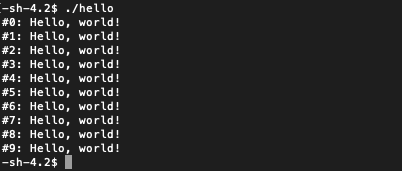
\includegraphics[scale=0.7]{hello_world_qt_loop.png}
\caption{Hello world with qt\_loop}
\label{fig:hello_world_qt_loop}
\end{figure}

\subsection{Optimizing loop execution}

If the amount of work performed in each iteration of a loop is uniform, more optimal performance typically may be achieved by dividing the iteration space into a number of qthreads equal to the number of available workers on the system, with each qthread containing an equal (or near equal) number of iterations.  The {\tt qt\_loop\_balance} API call offers this functionality.  Its use is shown in the following example:
\\
\lstinputlisting{examples/hello_world_loop_optimized.c}

The only change to the code from the previous example is that the call has been changed from {\tt qt\_loop} to {\tt qt\_loop\_balance}.  The arguments to both calls are the same.  The internal implementation of {\tt qt\_loop\_balance} in the Qthreads run time system performs the division of the iteration space into qthreads based on the number of available workers.  Thus, the same code may be executed on systems with different numbers of hardware threads, or on different numbers of threads on the same machine, without any changes to the code.
\\ \\
{\footnotesize{\tt cc -o hello -I\$QTHREAD\_INC -L\$QTHREAD\_LIB -lqthread hello\_world\_loop\_optimized.c}}
\\
{\footnotesize{\tt ./hello}}
\begin{figure}[h]
\includegraphics[scale=0.85]{hello_world_optimized.png}
\caption{Hello world with qt\_loop\_balance}
\end{figure}

\section{Atomics and Blocking}

Qthreads has a number of tools for doing atomic and blocking operations. An
illustrative example of a non-blocking atomic operation is the {\tt
qthread\_incr} function. The increment function is a thread-safe version of
{\tt *operand += incr;}
In the following program we have a number of tasks that all increment a single
variable, with the desired property that the variable is incremented {\tt n}
times.
\\
\lstinputlisting{examples/incr.c}
{\footnotesize{\tt cc -o incr -I\$QTHREAD\_INC -L\$QTHREAD\_LIB -lqthread incr.c}}
\\
{\footnotesize{\tt ./incr}}
\begin{figure}[h]
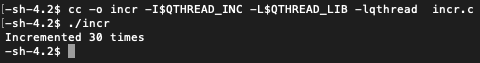
\includegraphics[scale=0.85]{incr.png}
\caption{Code showing usage of atomic function qthread\_incr}
\end{figure}

\newpage
\subsection{Barriers}

Qthreads has a number of mechanisms for creating barriers as well. For example,
we could implement the above incrementer using a barrier instead of the {\tt
readFF} function calls.

Instead of the parent task blocking on each full empty bit in order, each task
is blocked until all tasks have entered the barrier. Then each is allowed to
continue, including the parent task. Note because we want the parent task to
wait on the barrier as well, the first argument (which is the number of tasks we
want to wait on) is {\tt n+1}.
\\
\lstinputlisting{examples/barrier.c}
{\footnotesize{\tt cc -o barrier -I\$QTHREAD\_INC -L\$QTHREAD\_LIB -lqthread barrier.c}}
\\
{\footnotesize{\tt ./barrier}}
\begin{figure}[h]
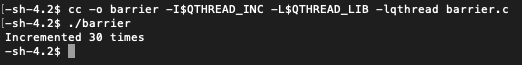
\includegraphics[scale=0.85]{barrier.png}
\caption{Code showing usage of barrier function}
\end{figure}

\newpage
\section{Calculating a Fibonacci number}

The following example illustrates naive brute-force calculation of the {\it n}-th Fibonacci number using recursive task parallelism. The program begins by generating a single qthread to execute the {\tt fib} function with the argument indicating which Fibonacci number ({\tt n}) to calculate.  The {\tt fib} function then calls itself recursively with arguments {\tt n-1} and {\tt n-2} until the base case of the recursion is satisfied. The program keeps track of the total number of created
\\
{\footnotesize{\tt cc -o fib -I\$QTHREAD\_INC -L\$QTHREAD\_LIB -lqthread fib.c}}
\\
{\footnotesize{\tt time ./fib}}
\\
{\footnotesize{\tt time ./fib 24}}
\lstinputlisting{examples/fib.c}
\begin{figure}[h]
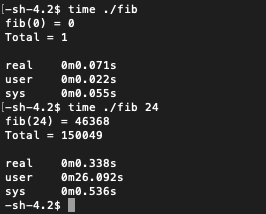
\includegraphics[scale=0.96]{fib.png}
\end{figure}

\subsection{A faster Fibonacci}
The program in the previous example generates a single qthread to execute each addition in the Fibonacci calculation.  Since the generation and execution of each qthread has an associated overhead cost, it is not recommended to perform so little computational work in each qthread.  In the following example program, a sequential calculation is introduced below a certain threshold. Because far fewer qthreads are created to solve a given problem, time spent on overhead costs is greatly reduced compared to the previous example program.
\\  \\
{\footnotesize{\tt cc -o fib -I\$QTHREAD\_INC -L\$QTHREAD\_LIB -lqthread fib\_fast.c}}
\\
{\footnotesize{\tt time ./fib}}
\\
{\footnotesize{\tt time ./fib 24}}

\begin{figure}[h]
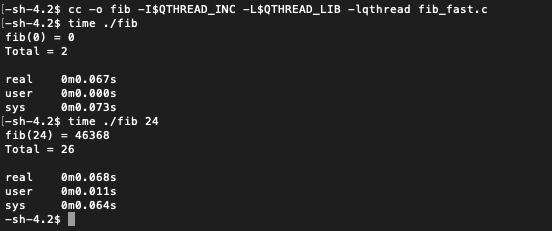
\includegraphics{images/fib_fast.png}
\end{figure}
\newpage
\lstinputlisting{examples/fib_fast.c}

\subsection{Fibonacci by preconditioned tasks}

Many algorithms can be structured as a set of qthreads partially ordered by dependence relationships.  Qthreads represents dependences between qthreads in terms of {\it preconditions}.  The following example program demonstrates their use.
\\
\lstinputlisting{examples/fib_preconditioned.c}

The code first defines two structure types, {\tt f\_arg\_t} and {\tt fr\_arg\_t}.  Pointers to structures of these types will be passed as arguments to the two functions {\tt fib\_result} and {\tt fib}, respectively.  We will examine these functions in reverse order.  The arguments provided to the {\tt fib} function specify the Fibonacci number to calculate ({\tt n}) and a location where the result will be placed ({\tt result}).   These arguments are unpacked from the {\tt arg} structure into local variables.  Unless {\tt n} is trivial, the remaining code in the function sets up and generates new qthreads to recursively call the {\tt fib} function and to combine the results using the {\tt fib\_result} function.  A new argument structure {\tt fibs} is allocated for the call to {\tt fib\_result}, and that structure contains within it an array of two argument structures for calls to {\tt fib}.  Pointers to these two structures are saved, their input fields are set to {\tt n-1} and {\tt n-2}, and the result fields are set to empty.  The second field of the {\tt fibs} argument structure is the target location where the sum of the combined results will be placed.  This is set to the {\tt result} field of {\tt fib}.

The {\tt qthread\_fork\_precond} API call generates a qthread to execute the {\tt fib\_result} function only when its preconditions are fulfilled.  The first three arguments to the call are the same as those of {\tt qthread\_fork}: the function, the pointer to the argument data to be passed to the function, and a pointer to the return value.  This example program collects the results through pointers in the argument structures, and thus does not use the third argument.  The fourth argument specifies the the number of preconditions that must be fulfilled before the run time will schedule for execution.  The remaining arguments specify those preconditions, in this case, the completion of the two recursive calls to {\tt fib}.  The {\tt qthread\_fork\_precond} call is followed by the two calls to {\tt qthread\_fork} that generate those recursive calls to {\tt fib}.  At this point, the function returns.  Thus the qthread executing {\tt fib} at run time does not wait for the recursive calls to complete.  Instead, the qthread generated to execute {\tt fib\_result} waits on the recursive calls, only beginning execution once they are finished.

Finally, we have the code for the {\tt main} function of the program, which is similar to that of the previous program.  The primary difference is that an argument structure is initialized for the first {\tt fib} task.  The {\tt n} field takes the Fibonacci number to be calculated, as specified by the command line argument.  The {\tt result} field is initially zero, and at the completion of all the qthreads generated, it contains the final result.
%:
\\ \\
{\footnotesize{\tt cc -o fib -I\$QTHREAD\_INC -L\$QTHREAD\_LIB -lqthread fib\_preconditioned.c}}
\\
{\footnotesize{\tt time ./fib}}
\\
{\footnotesize{\tt time ./fib 24}}
\newpage
\lstinputlisting{examples/fib_preconditioned.c}

\begin{figure}
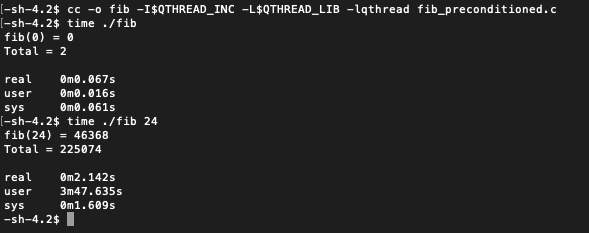
\includegraphics{images/fib_preconditioned.png}
\end{figure}


\section{Accumulators and Reductions}
One common design pattern is that of an \emph{accumulator} or a
\emph{reduction}. These are used when we want to reduce a large amount of data
to a value. For example, one might want to compute the maximum value from a
large number array. There is a function for this kind of approach in qthreads
called {\tt qt\_loopaccum\_balance}. A simple example of using {\tt
qt\_loopaccum\_balance} is given below, which computes the sum of an array.
\\

\lstinputlisting{examples/loopaccum_balance.c}

The work is broken up into chunks, then each chunk is summed in the {\tt
qtds\_worker} function, and then the sums are reduced using {\tt qtds\_acc}.
Both the worker and the accumulator functions will be assigned to workers
automically by the qthreads runtime. Note the types of the arguments for the
worker. The second argument is {\tt const}, to make it clear that the value must
be accumulated in the location pointed to by the first argument. 

\subsection{Sincs}
There may be use cases when you want to write your own reduction. For example,
perhaps you might need some sort of tree-reduction. One tool in the qthreads
toolbox that can be helpful for this sort of application is the sinc. In the
following example, we use sincs to build an {\tt n}-ary tree of deth {\tt d}
and sum the leaves in parallel.
\\

\lstinputlisting{examples/sinc.c}

The sinc structure contains a function that works similarly to the function
bound in the loopaccum example. The first argument is a pointer to the
accumulator, and the second is a pointer to the value we want to accumulate.
Note we create a new sinc at each node in the tree, waiting on its children. The
{\tt qt\_sinc\_submit} function applies the accumulator function, in this case,
{\tt incr} and adjusts the semaphore in the sinc structure such that when the
correct number of submissions have been made (in this case {\tt n}), any threads
waiting on the sinc (in this case only one) can continue.

\newpage
\section{Workers and Shepherds}

As described in the introduction, the workers are usually bound one per core,
while the shepherds (shared work queues) are often bound somewhere higher in the
memory hierarchy. While qthreads will try and do The Right Thing$^{\circledR}$,
there may be times where the user needs to set the number of workers or
shepherds. The recommended way to do this is with environment variables. For
example: running with {\tt QT\_NUM\_SHEPHERDS=8
QT\_NUM\_WORKERS\_PER\_SHEPHERD=2} will yield 8 shepherds and 16 workers. You
can check the number of workers and shepherds with the api calls {\tt
qt\_num\_workers()} and {\tt qt\_num\_shepherds()}. For example:

\lstinputlisting{examples/numworksheps.c}

\subsection{Worker ID}

While not recommended for most use cases, there may be situations where one
would want to use worker id explicitly. In the following example, we again do a
simple sum reduction, this time explicitly taking into account the number of
workers, and assigning each worker to a subset of the array to be summed.

\lstinputlisting{examples/worker_id.c}

\newpage
\section{High Performance Asyncronous Behaviour}

One application of lightweight threads is low overhead asynchronous behaviour.
For example, if we want a server to do some expensive computation
asynchronously, qthreads is a good option. In the following example, we have a
tcp server that reads in an integer and computes the fibonacci sequence at that
index. While this could be done with a fork or pthread, this approach will allow
significantly higher throughput by reducing the overhead of spawning the task.  

\lstinputlisting{examples/tcpserver.c}

Note there is an unfamiliar API call here as well: {\tt qthread\_flushsc}. The
current default behaviour is to buffer tasks before moving them into the queue.
This flushes said buffer, which is necessary in cases like this to begin work.
To test this example, simply telnet or netcat to localhost port 5000 and
enter some numbers (remember it's naive fibonacci, so don't enter large numbers
if you want a result!). To get interesting asynchronous behaviour, responses will
likely start slowing down around {\tt n = 40}.

% TODO: yield, spawn cache

\end{document}
